\section{Slides de Aulas}

A melhor estratégia para o estilo dos slides de aula são o fundo branco, letras escuras, e cores para ressaltar. Isso se adequa bem tanto a salas bem iluminadas quanto a salas escuras, para todo tipo de projetor. A Figura \ref{fig:teximag}, apesar de usar o forte grená, me parece bastante adequada. As outras figuras  mostram outros modelos que eu uso e sinto adequados para uma aula. As cores azuis e cinzas, porém, são mais ``fracas'' e podem levar a um pouco de monotonia.

\begin{figure}[hbt]
    \centering
    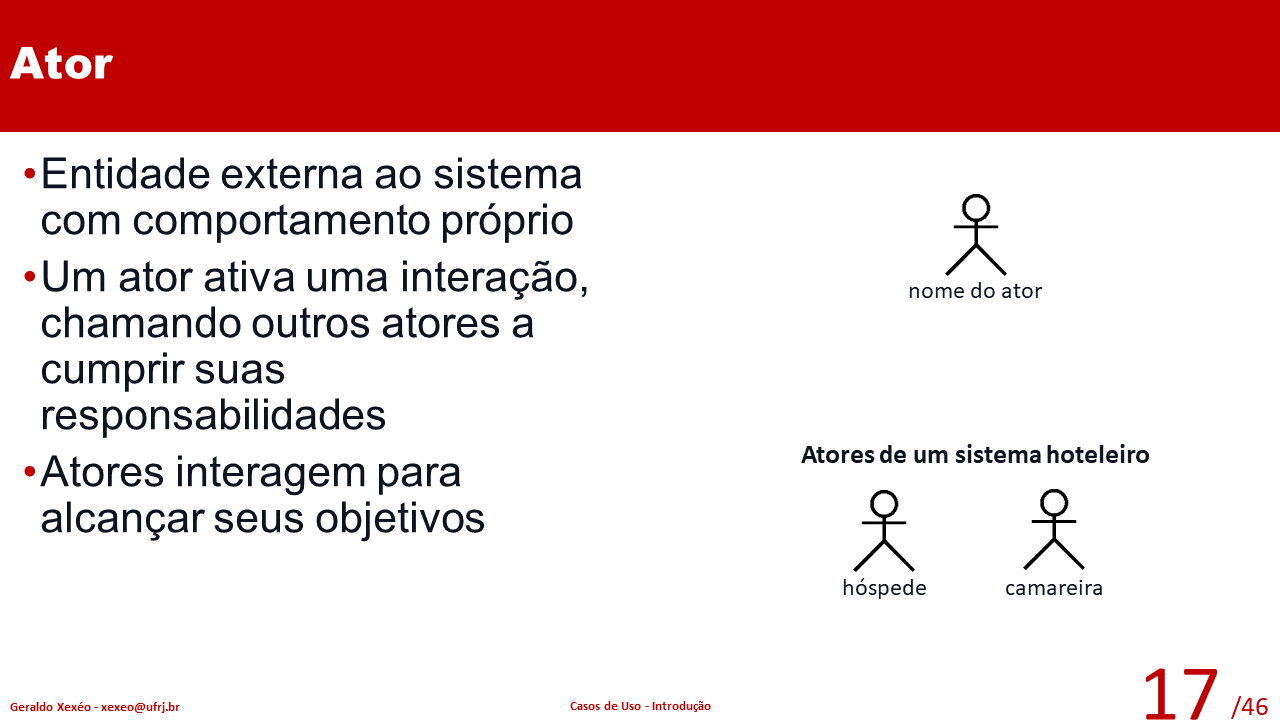
\includegraphics[width=\tam\linewidth]{imagens/slidecomimage.png}
    \caption{Slide com texto e imagem}
    \label{fig:teximag}
\end{figure}

